\begin{exercise}{1}
	In this problem we look at different dynamical systems using software written by Rice Professor John C. Polking. The software is pplane, and allows us to graph the phase planes of dynamical systems.
	\\
	\\
	\textbf{Results}\\
	The first system we look at is 
	\[\frac{d}{dt} \begin{pmatrix} x \\ v\\ \end{pmatrix} = 
	  \begin{pmatrix}
	  	0 & 1\\
	  	-k/m & -d/m \\
	  \end{pmatrix}
	  \begin{pmatrix}
	  	x \\ v\\
	  \end{pmatrix}
	\]
	When $d = 0$, we have a system with solutions that circle around the origin. When we have $d = 1$, the system's solutions start to spiral in toward the origin.

	The second system that we look at is give by Van der Pol's Equation. With a default parameter $M = 2$ we get the following system \\

	\begin{figure}[!h]
		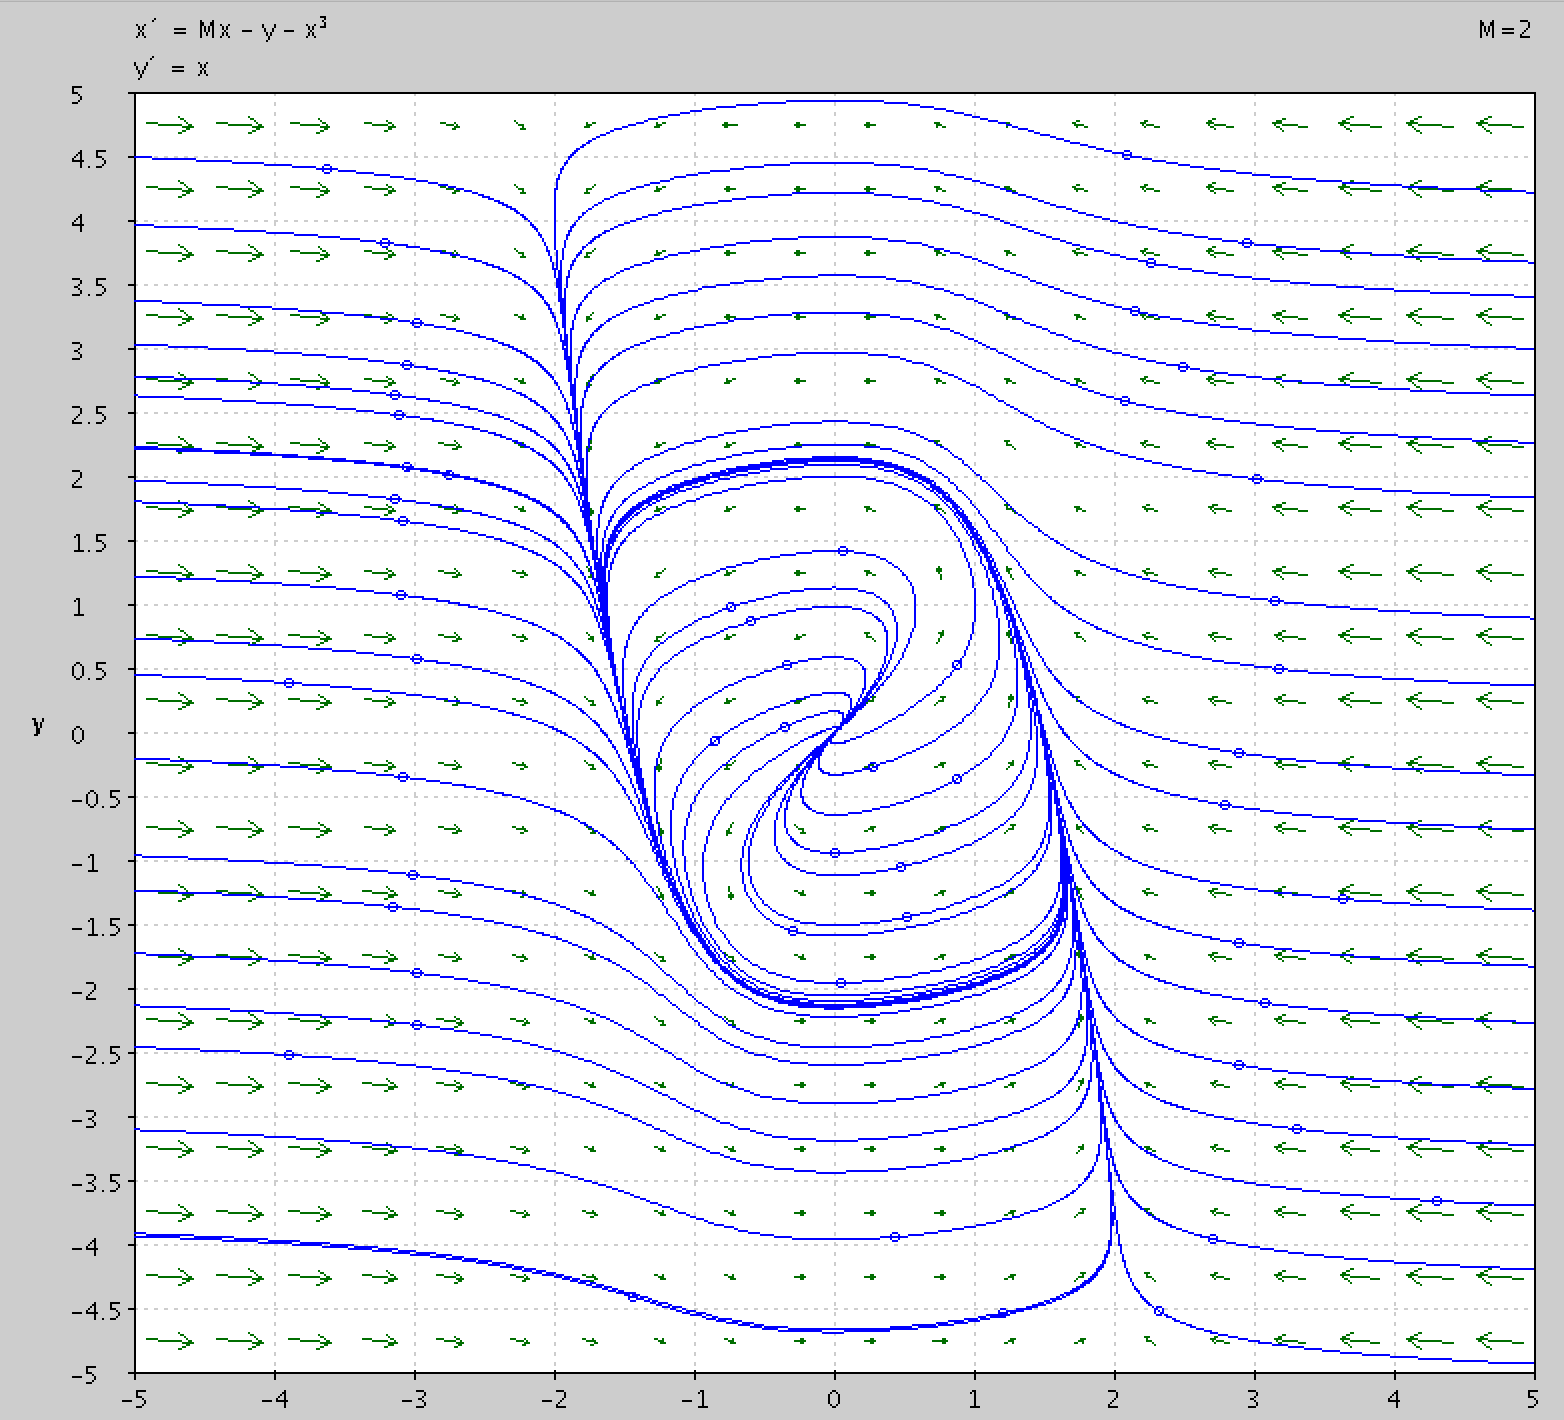
\includegraphics[width=300px]{graph1.png}
	\end{figure}
	The solutions tend toward what is known as a limit cycle. You can see that there is an isolated closed trajectory. Solutions that start outside of this closed trajectory approach the trajectory, and solutions that start on the inside of the closed loop spiral out from the origin toward the loop.
\end{exercise}